\section{Model Acceleration}
\label{sec:accelerate}

\begin{figure}[htbp]
    \centering
    \begin{subfigure}[b]{0.28\textwidth} % 左边的子图占60%
        \centering
        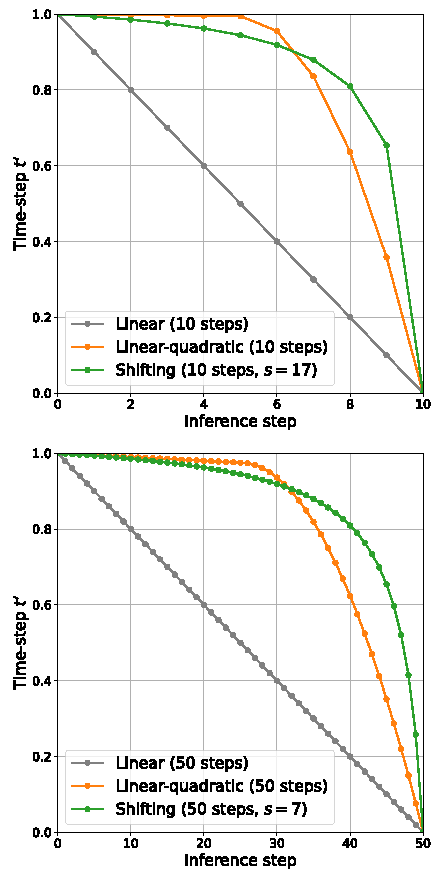
\includegraphics[width=\textwidth]{figures/shifting.pdf}
        \caption{}
        \label{fig:shifting}
    \end{subfigure}
    \hfill
    \begin{subfigure}[b]{0.69\textwidth} % 右边的子图占40%
        \centering
        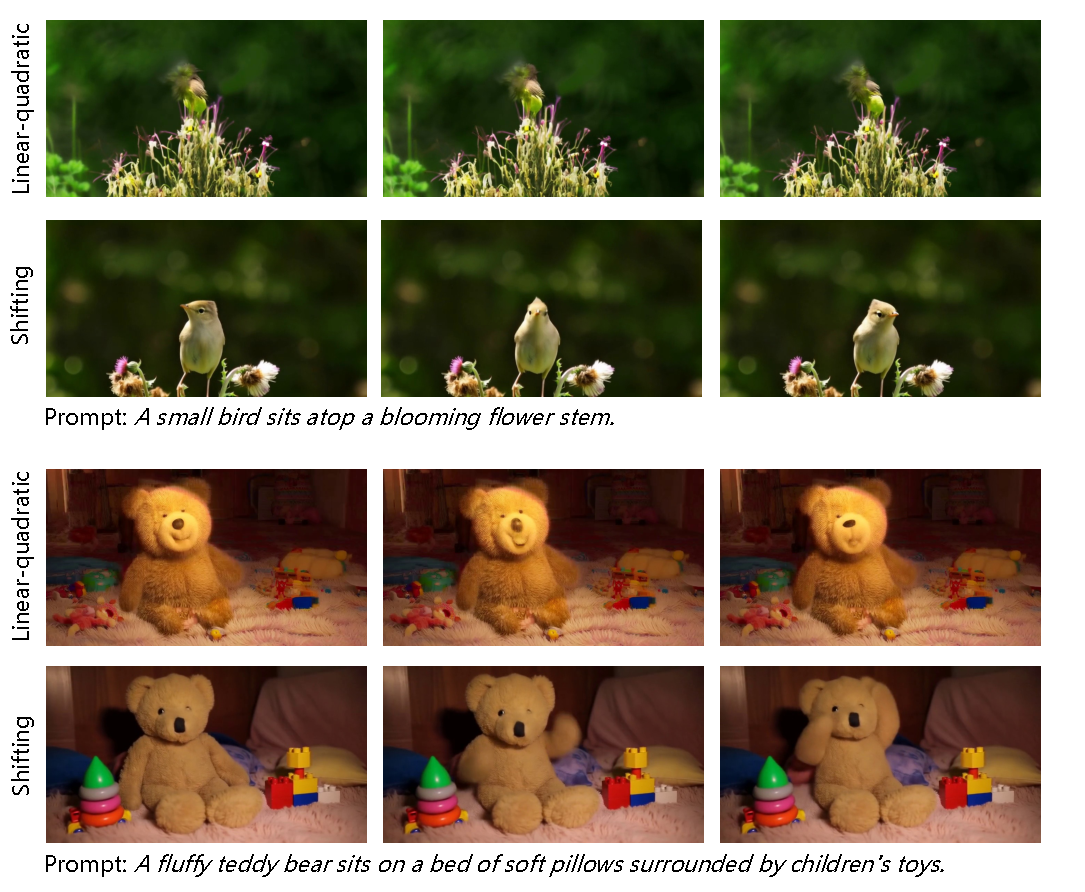
\includegraphics[width=\textwidth]{figures/shifting_example.pdf}
        \caption{}
        \label{fig:shifting_example}
    \end{subfigure}
    \caption{(a) Different time-step schedulers. For our shifting stragty, we set a larger shifting factor $s$ for a lower inference step. (b) Generated videos with only 10 inference steps. The shifting stragty leads to significantly better visual quality.}
    \label{fig:overall}
\end{figure}


\subsection{Inference Step Reduction }
% \dq{@Common Utility Team}

To improve the inference efficiency, we firstly consider reducing the number of inference steps. Compared to image generation, it is more challenging to maintain the spatial and temporal quality of the generated videos with lower inference steps. Inspired by a previous observation that the first time-steps contribute to most changes during the generation process \cite{zhao2024real,polyak2024movie,zhang2022unsupervised,zhang2023shiftddpms}, we utilize the time-step shifting to handle the case of lower inference steps. Specifically, given the inference step $q \in \{1,2,...,Q\}$, $t=1-\frac{q}{Q}$ is the input time condition for the generation model, where the noise is initialized at $t=1$ and the generation process halts at $t=0$. Instead of using $t$ directly, we map $t$ to $t'$ with a shifting function $t'=\frac{s*t}{1+(s-1)*t}$, where $t'$ is the input time condition and $s$ is the shifting factor. If $s>1$, the flow model is conditioned more on early time steps. A critical observation is that a lower inference step requires a larger shifting factor $s$. Empirically, $s$ is set as 7 for 50 inference steps, while $s$ should be increased to 17 when the number of inference steps is smaller than 20. The time-step shifting strategy enables the generation model to match the results of numerous inference steps with a reduced number of steps.

MovieGen \cite{polyak2024movie} applies the linear-quadratic scheduler to achieve a similar goal. The schedulers are visualized in Figure \ref{fig:shifting}. However, we find that our time-step shifting is more effective than the linear-quadratic scheduler in the case of extremely low number of inference steps, $e.g.$, 10 steps. As shown in Figure \ref{fig:shifting_example}, the linear-quadratic scheduler results in worse visual quality. 
 

\subsection{Text-guidance Distillation}
% \dq{@Common Utility Team}

Classifier-free guidance (CFG) \cite{ho2022classifier} significantly improves the sample quality and motion stability of text-conditioned diffusion models.
%However, it increases computational cost and inference latency since it computes the output for the unconditional input except for the conditional one at each inference step.
However, it increases computational cost and inference latency since it requires extra output for the unconditional input at each inference step.
%Generally, the unconditional and conditional inferences are implemented in a single batch in parallel.
Especially for the large video model and high-resolution video generation, the inference burden is extremely expensive when generating text-conditional and text-unconditional videos, simultaneously.
%Due to the great number of parameters and long-context lengths for our video generation model, the need for additional computation and memory becomes more notable. 
To solve this limitation, we distill the combined output for unconditional and conditional inputs into a single student model \cite{meng2023distillation}.
Specifically, the student model is conditioned on a guidance scale and shares the same structures and hyper-parameters as the teacher model.
We initialize the student model with the same parameters as the teacher model and train with the guidance scale randomly sampled from 1 to 8. We experimentally find that text-guidance distillation approximatively brings 1.9x acceleration. 

\subsection{Efficient and Scalable Training}
% \dq{@Infra Team}

% \subsubsection{Overview}
To achieve scalability and efficient training, 
we train \nameofmethod{} on AngelPTM \cite{nie2023angel}, 
the large-scale pretraining framework from Tencent Angel machine learning team.
In this part, we first outline the hardware and infrastructure used for training, and then give a detailed introduction to the model parallel method and its optimization methods, followed by the automatic fault tolerance mechanism.

\subsubsection{Hardware Infrastucture}
% \nameofmethod{} uses NVIDIA GPUs to complete the entire training pipeline.
To ensure efficient communication in large-scale distributed training, we setup a dedicated distributed training framework termed Tencent XingMai network \cite{2024tccl} for highly efficient inter-server communication. 
The GPU scheduling for all training tasks is completed through the Tencent Angel machine learning platform, which provides powerful resource management and scheduling capabilities.

\subsubsection{Parallel Strategy}
\nameofmethod{} training adopts 5D parallel strategies, including tensor parallelism (TP) \cite{2019megatron}, sequence parallelism (SP) \cite{2022sequence-parallelism}, context parallelism (CP) \cite{2024context-parallelism}, and data parallelism combined with Zero optimization (DP + ZeroCache \cite{nie2023angel}).
The tensor parallelism (TP) is based on the principle of block calculation of matrices. The model parameters (tensors) are divided into different GPUs to reduce GPU memory usage and accelerate the calculation. Each GPU is responsible for the calculation of different parts of tensors in the layer.

Sequence parallelism (SP) is based on TP. The input sequence dimension is sliced to reduce the repeated calculation of operators such as LayerNorm and Dropout, and reduce the storage of the same activations, which effectively reduces the waste of computing resources and GPU memory.
In addition, for input data that does not meet the SP requirements, the engineering equivalent SP Padding capability is supported.

Context parallelism (CP) is sliced in the sequence dimension to support long-sequence training. Each GPU is responsible for calculating the Attention of different sequence slices. Specifically, Ring Attention \cite{2023ring-attention} is used to achieve efficient training of long sequences through multiple GPUs, breaking through the GPU memory limitation of a single GPU.

In addition, data parallelism + ZeroCache is leveraged to support horizontal expansion through data parallelism to meet the demand for increasing training data sets. Then, based on data parallelism, the ZeroCache optimization strategy is used to further reduce the redundancy of model states (model parameters, gradients, and optimizer states), and we unify the use of GPU memory to maximize the GPU memory usage efficiency.

\subsubsection{Optimization}
\textbf{Attention optimization.} 
As the sequence length increases, the attention calculation becomes the main bottleneck of training. We accelerated the attention calculation with FusedAttention.

\textbf{Recomputation and activations offload optimization.} Recomputation is a technology that trade calculations for storage. 
It is mainly made up of three parts: a) specifying certain layers or blocks for recalculation, b) releasing the activations in the forward calculation, and c) obtaining the dependent activations through recalculation in the backward calculation, which significantly reduces the use of GPU memory during training.
In addition, considering the PCIe bandwidth and the host memory size, a layer-based activation offload strategy is adopted. Without reducing the training performance, the activations in the GPU memory are offloaded to the host memory, further saving GPU memory.

\subsubsection{Automatic fault tolerance}
In terms of the large-scale training stability of \nameofmethod{}, an automatic fault tolerance mechanism is used to quickly restore training for common hardware failures.
This avoids frequent occurrence of the manual recovery of training tasks.
%, which  due to failure to the recovery of the training task is in minutes.
By automatically detecting errors and quickly replacing healthy nodes to pull up training tasks, the training stability is 99.5\%.